\clearpage{\pagestyle{empty}\cleardoublepage}

\chapter{Risultati ottenuti}

\begin{flushright}\begin{small}\textit{"Hard science gives sensational results\\ with a horribly boring process."}\\
- Nassim Nicholas Taleb -\\
\end{small}\end{flushright}

Lo sviluppo e la convalida dell'algoritmo sono stati permessi grazie all'utilizzo di quest'ultimo per la correzione di immagini in fluorescenza rossa di cellule di fibroblasti, sfruttando apposite immagini di calibrazione di sferette, anch'esse fluorescenti nel rosso.

Le immagini di riferimento, utilizzate nella prima e nella seconda fase del programma, sono state acquisite in otto pozzetti di una multiwell: due con sferette ad intensità relativa del 100\% e due del 10\%, due con una mixture di cinque intensità (1\%, 3\%, 10\%, 30\% e 100\%) ed infine nelle rimanenti è stato posto unicamente il mezzo di coltura, così da studiare la fluorescenza di background indotta dalla sorgente.
Il riempimento di ogni pozzetto ha previsto l'agitazione sia manuale che con sonificatore delle sferette e l'iniezione con le pipette ghilson di $220\ \mu l$ di terreno completo e delle sferette di calibrazione: $10\ \mu l$ per i quattro pozzetti ad intensità unica e $2\ \mu l$ per i due pozzetti a cinque intensità.
Tuttavia una delle due immagini con sferette aventi differente luminosità ha mostrato un'errata composizione del campione e perciò ai fini dell'elaborazione dati se ne è sfruttata una sola di queste.

L'analisi che segue pone in particolare l'attenzione sull'efficacia dell'algoritmo nella rimozione dell'``effetto dei bordi'' poiché, come visto in precedenza, il difetto della fluorescenza di sfondo viene semplicemente eliminato sottraendo il parametro costante identificato nella seconda fase.

Tale capitolo si propone di esporre e commentare i risultati conseguiti dall'algoritmo, i quali possono essere raccolti da differenti analisi: l'osservazione degli istogrammi delle distribuzioni di intensità, il cambiamento sostanziale del p-value associato alla dipendenza spaziale della luminescenza e la semplice analisi qualitativa dell'evoluzione delle immagini durante le varie fasi di correzione.
Queste tre rielaborazioni verranno affrontate sulla base di grafici e risultati ottenuti applicando l'algoritmo sull'immagine dei fibroblasti, nel particolar caso in cui la prima immagine di calibrazione sia costituita da un campione di sferette con intensità relativa del 10\%.
Successivamente, per poter avere una miglior valutazione dell'efficacia del programma, verrà eseguito un confronto tra i risultati ottenuti utilizzando nella prima fase dell'algoritmo quattro distinte immagini di calibrazione, acquisite col microscopio a fluorescenza.

Osserviamo inoltre che prima di giungere ai risultati finali di seguito riportati l'algoritmo è stato via via migliorato: ad esempio, si è constatato che la curva in grado di fittare al meglio i centri di sferette nella prima fase dell'algoritmo fosse, anziché una polinomiale, una curva di tipo esponenziale, che l'intensità da associare ad ogni punto di massimo fosse meglio interpretarla come intensità integrale media piuttosto che puntuale ed inoltre sono stati ricavati ed inseriti i valori ottimali dei parametri utilizzati nei vari passaggi di elaborazione dell'immagine.

\section{Distribuzione delle intensità}

Come visto, l'``effetto dei bordi'' consiste nel fatto che il microscopio crei immagini con intensità maggiore al centro rispetto al margine, comportando di conseguenza un'alterazione della distribuzione delle intensità. 
Tale fenomeno viene attenuato in modo sostanziale tramite l'azione della prima fase dell'algoritmo, la quale agisce proprio sul difetto preso in considerazione.

Il cambiamento della distribuzione di intensità provocato dal software è percepibile graficando gli istogrammi relativi alle varie intensità rilevate all'interno dell'immagine in fase pre e post correzione.

Il miglioramento più evidente da questo punto di vista si ha nell'istogramma della prima immagine di calibrazione (\figurename~\ref{fig:isto1}), poiché le intensità, prima distribuite entro un range molto ampio, risultano molto più piccate attorno un unico valore.
Tale risultato è proprio ciò a cui si mirava, dato che le sferette contenute nel campione risultano avere la medesima intensità.

Anche in \figurename~\ref{fig:isto2} si nota un netto miglioramento, infatti le cinque gaussiane associate ai differenti valori di intensità relativa delle sferette mostrano a posteriori dell'elaborazione un'apertura, ossia una covarianza, molto minore ed una miglior definizione dei confini tra l'una e l'altra. 

D'altra parte, gli istogrammi associati all'immagine volta a correzione (\figurename~\ref{fig:isto3}), ovvero quella delle cellule, non presentano sostanziali cambiamenti, a meno di una migliore simmetria della distribuzione delle intensità presenti nell'immagine.
Tale risultato era in realtà prevedibile, dato che in tal caso non si tratta più di un'immagine di calibrazione, quindi creata per poter mostrare determinate proprietà luminescenti, bensì di un'immagine reale e di natura biologica. 
Per tale motivo le intensità rilevate nell'immagine è giusto che si estendano entro un range abbastanza ampio, proprio perché a seconda della concentrazione delle probes fluorescenti nella cellula sarà differente il grado di luminosità sviluppato.

\begin{figure}
 \centering
 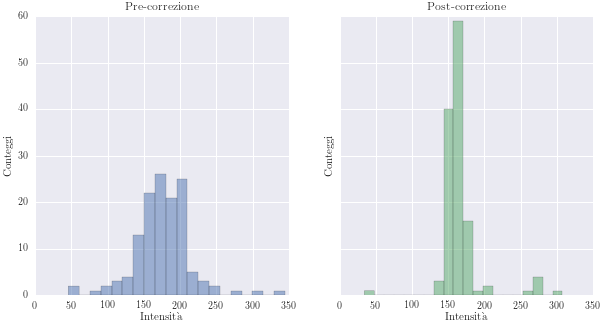
\includegraphics[scale=.55]{img/CAP4isto1.png}
 \caption{\small{Istogrammi relativi alle intensità dei massimi della prima immagine di calibrazione, costituita da sferette con stessa intensità. Il grafico a sinistra è associato alla fase di pre-correzione (\figurename~\ref{fig:unaint}), mentre quello a destra alla fase di post-correzione (\figurename~\ref{fig:unaintcorr}). Come previsto, l'algoritmo di correzione fa sì che le intensità risultino molto più piccate attorno un unico valore.}}
 \label{fig:isto1}
\end{figure}

\begin{figure}
 \centering
 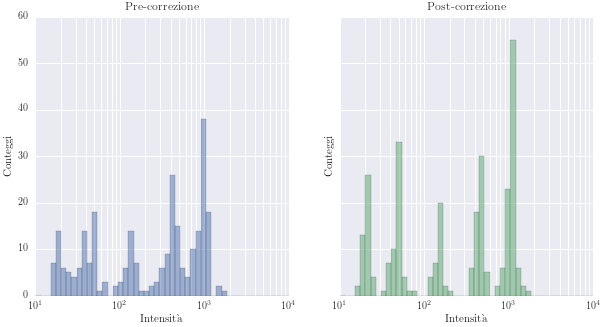
\includegraphics[scale=.55]{img/CAP4isto2.png}
 \caption{\small{Istogrammi relativi alle intensità dei massimi della seconda immagine di calibrazione, costituita da sferette con cinque intensità differenti. Il grafico a sinistra è associato alla fase di pre-correzione (\figurename~\ref{fig:piuint}), mentre quello a destra alla fase di post-correzione (\figurename~\ref{fig:piuintcorr}). Come previsto, l'algoritmo di correzione fa sì che le intensità risultino molto più piccate attorno ai cinque valori medi delle gaussiane, rendendo queste molto più definite.}}
 \label{fig:isto2}
\end{figure}

\begin{figure}
 \centering
 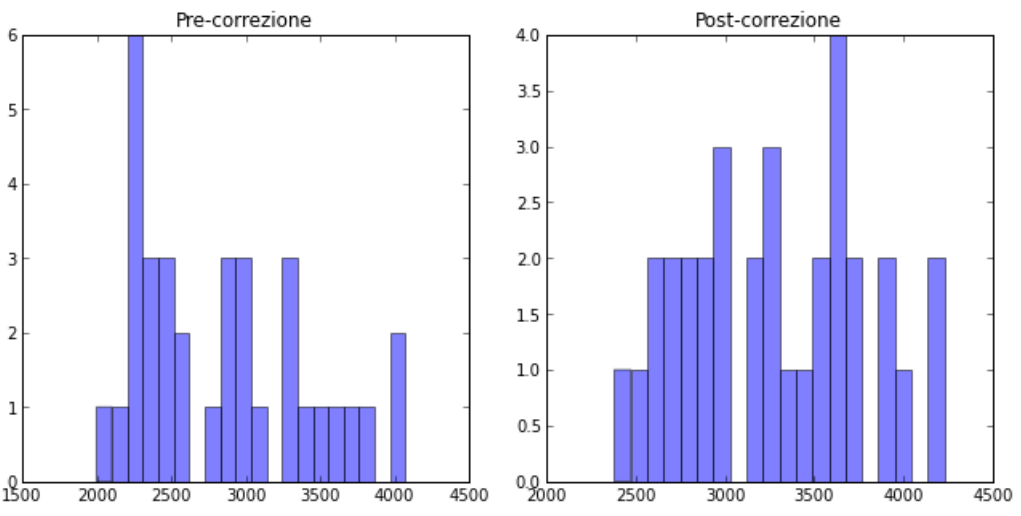
\includegraphics[scale=.55]{img/CAP4isto3.png}
 \caption{\small{Istogrammi relativi alle intensità dei massimi dell'immagine delle cellule di fibroblasti. Il grafico a sinistra è associato alla fase di pre-correzione (\figurename~\ref{fig:cell}), mentre quello a destra alla fase di post-correzione (\figurename~\ref{fig:cellcorr}). Come previsto, l'algoritmo di correzione determina una miglior simmetria della distribuzione di intensità.}}
 \label{fig:isto3}
\end{figure}


\section{Dipendenza spaziale dell'intensità}

In statistica, data un'ipotesi nulla ($H_0$), questa la si può accettare o rifiutare sulla base del cosiddetto \textit{p-value}, parametro probabilistico con valore compreso tra 0 ed 1.
Esso può essere definito come livello di significatività assegnato e quantifica la ``forza dell'evidenza'' contro l'ipotesi nulla $H_0$, a favore dell'alternativa, espressa dai dati osservati su un determinato campione. 
Per esempio, assegnato un valore di soglia, se il p-value è maggiore di tale valore allora $H_0$ non viene rigettata, in caso contrario sì.
Di conseguenza il p-value esprime quanto sia plausibile che i dati osservati si ottengano essendo vera l’ipotesi nulla: un p-value grande esprime evidenza sperimentale a favore dell'ipotesi nulla, mentre un suo valore piccolo un'evidenza a favore dell'ipotesi alternativa.

Come precedentemente osservato, l'``effetto dei bordi'' comporta l'instaurarsi di una dipendenza dell'intensità del pixel dalla posizione di quest'ultimo: è proprio la ``forza'' di questa relazione funzionale che può essere misurata tramite il valore del p-value.
A tal proposito è stata valutata per ogni punto di massimo dell'immagine (centro delle sferette per le immagini di calibrazione e nuclei delle cellule per l'immagine da correggere) la distanza dall'origine, intesa come punto centrale dell'immagine stessa, così da ottenere un set di dati costituito da una sorta di distanze radiali. 
Per ottenere il valore del p-value si è quindi sfruttata la funzione \textit{linregress}, in grado di valutare la relazione lineare esistente o meno tra le intensità dei punti di massimo e le distanze radiali associate.
Tale funzione restituisce il p-value come semplice parametro di return e questo viene valutato prendendo come ipotesi nulla $H_0$ il fatto che la slope sia nulla, quindi maggiore sarà il p-value e più plausibile sarà assumere l'assenza di una dipendenza spaziale dell'intensità.

\begin{figure}
 \centering
 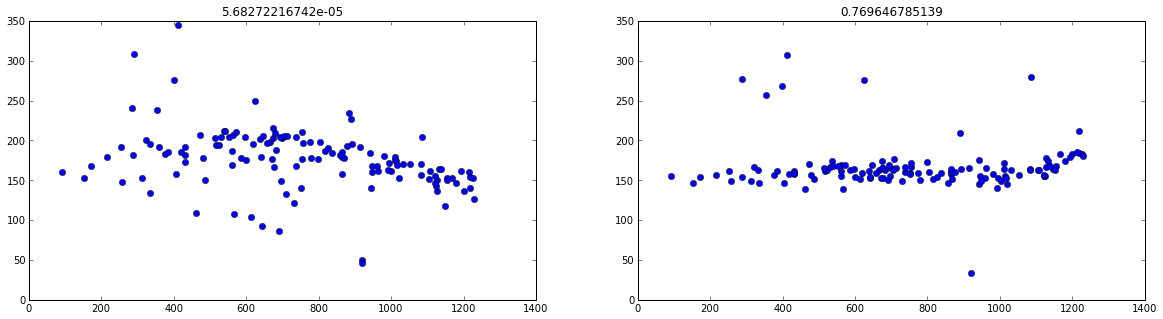
\includegraphics[scale=.55]{img/CAP4pvalue1.png}
 \caption{\small{Distribuzione delle intensità dei massimi in funzione della distanza radiale, relativa alla prima immagine di calibrazione. Il grafico a sinistra è associato alla fase di pre-correzione (\figurename~\ref{fig:unaint}), mentre quello a destra alla fase di post-correzione (\figurename~\ref{fig:unaintcorr}). In alto sono riportati i valori del p-value associato alla corrispondente regressione lineare. Come previsto, il p-value si avvicina ad 1 una volta applicato l'algoritmo sull'immagine.}}
 \label{fig:pvalue1}
\end{figure}

\begin{figure}
 \centering
 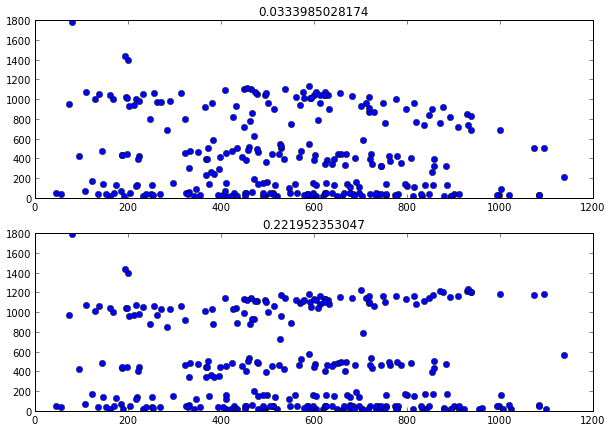
\includegraphics[scale=.55]{img/CAP4pvalue2.png}
 \caption{\small{Distribuzione delle intensità dei massimi in funzione della distanza radiale, relativa alla seconda immagine di calibrazione. Il grafico a sinistra è associato alla fase di pre-correzione (\figurename~\ref{fig:piuint}), mentre quello a destra alla fase di post-correzione (\figurename~\ref{fig:piuintcorr}). In alto sono riportati i valori del p-value associato alla corrispondente regressione lineare. Come previsto, il p-value si avvicina ad 1 una volta applicato l'algoritmo sull'immagine.}}
 \label{fig:pvalue2}
\end{figure}

\begin{figure}
 \centering
 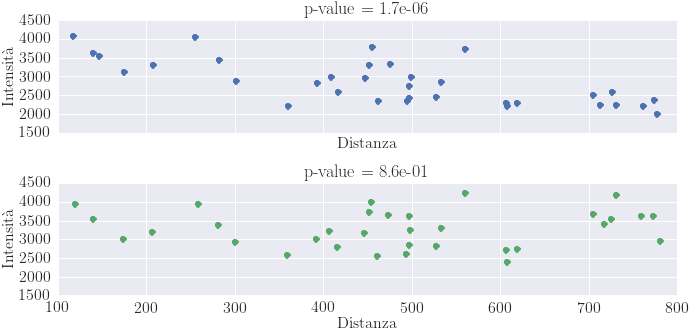
\includegraphics[scale=.55]{img/CAP4pvalue3.png}
 \caption{\small{
 Distribuzione delle intensità dei massimi in funzione della distanza radiale, relativa all'immagine delle cellule di fibroblasti. Il grafico a sinistra è associato alla fase di pre-correzione (\figurename~\ref{fig:cell}), mentre quello a destra alla fase di post-correzione (\figurename~\ref{fig:cellcorr}). In alto sono riportati i valori del p-value associato alla corrispondente regressione lineare. Come previsto, il p-value si avvicina ad 1 una volta applicato l'algoritmo sull'immagine.}}
 \label{fig:pvalue3}
\end{figure}

Come si evince dalle Figure \ref{fig:pvalue1}, \ref{fig:pvalue2}, \ref{fig:pvalue3}, il p-value viene altamente modificato dall'algoritmo e fatto crescere verso valori sempre più prossimi ad uno, comportando quindi una npiù piccola possibilità di correlazione esistente tra intensità e distanza radiale, sia nelle immagini di calibrazione che nell'immagine dei fibroblasti. 
Perciò, sulla base di tale analisi, dopo aver corretto l'immagine la dipendenza spaziale dell'intensità, inizialmente presente a causa della disomogeneità dell'illuminazione creata dalla sorgente, può essere considerata sostanzialmente non significativa.


\section{Analisi qualitativa delle immagini}

Anche dalla semplice osservazione delle immagini è possibile notare i cambiamenti apportati dall'algoritmo.

\begin{figure}
 \centering
 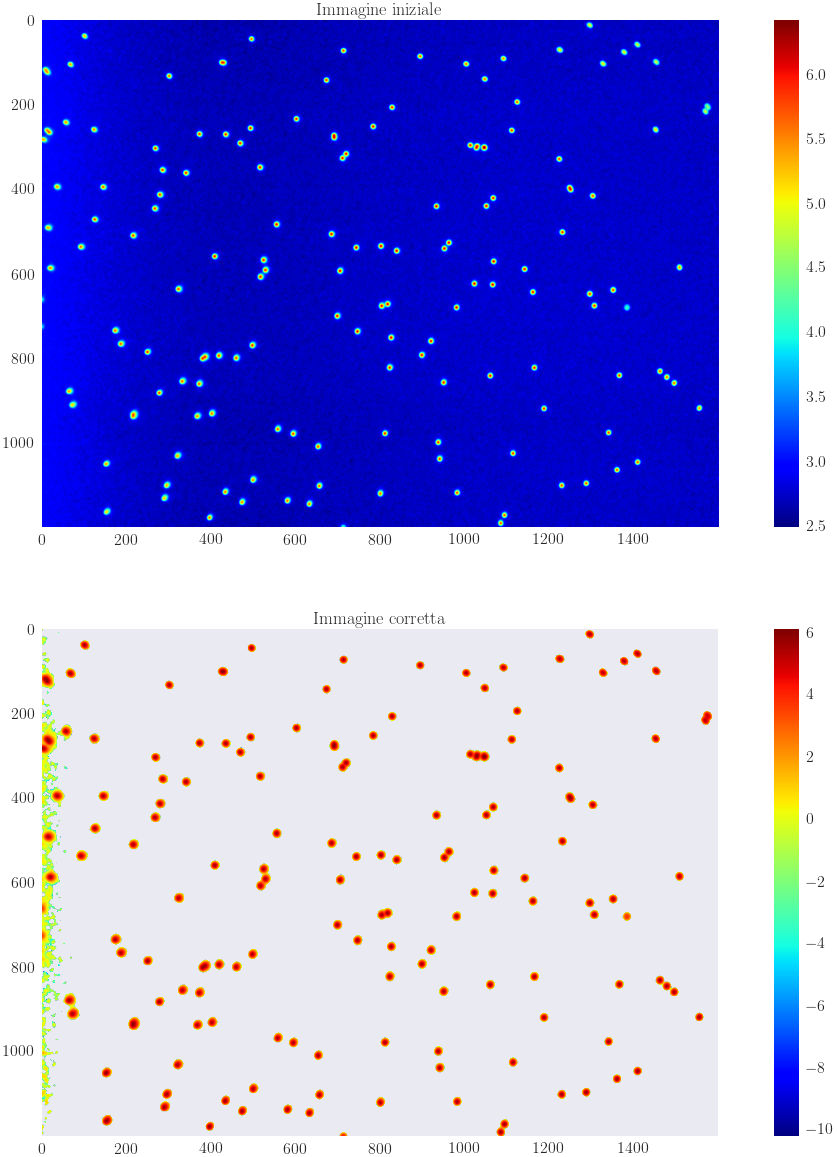
\includegraphics[scale=.40]{img/CAP4lg1.png}
 \caption{\small{Evoluzione della prima immagine di calibrazione: in alto è raffigurata l'immagine acquisita col microscopio a fluorescenza e in basso quella risultante dopo aver corretto l'``effetto dei bordi''. Le immagini, rappresentate nella color map ``jet'' riportata a fianco, sono i logaritmi delle corrispettive immagini originali, a cui è stato applicato ulteriormente il filtro gaussiano.}}
 \label{fig:lg1}
\end{figure}

In \figurename~\ref{fig:lg1} è possibile notare la sostanziale correzione del difetto della luminosità disomogenea: le sferette aventi stessa intensità, originariamente percepite con differente luminosità, vengono rappresentate dopo la correzione con una medesima tonalità di colore, mostrando così in modo più fedele la realtà del campione.

\begin{figure}
 \centering
 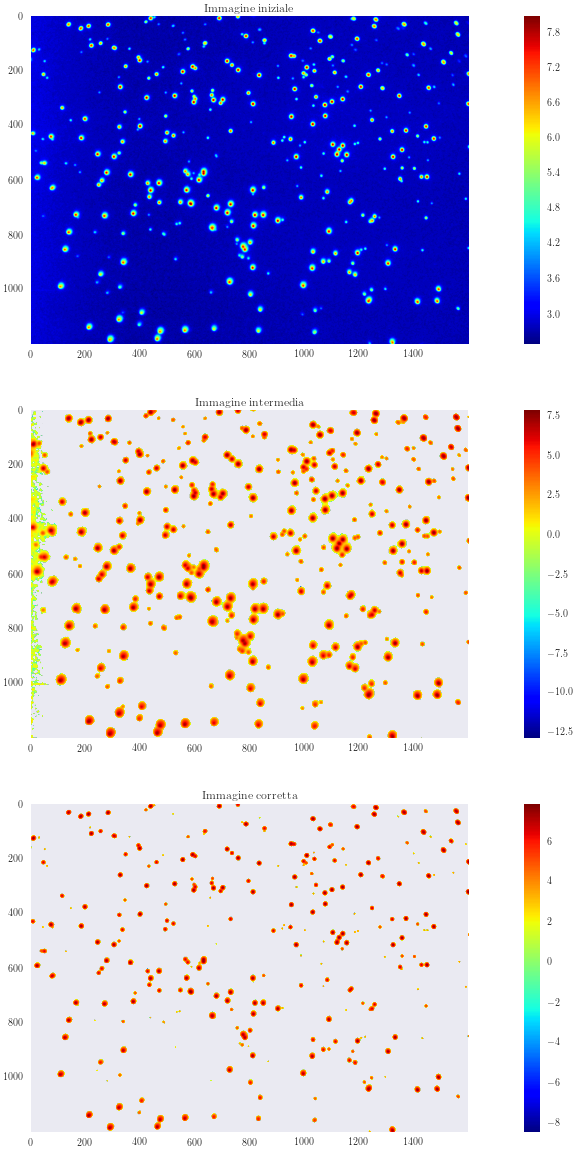
\includegraphics[scale=.50]{img/CAP4lg2.png}
 \caption{\small{Evoluzione della seconda immagine di calibrazione: in alto è raffigurata l'immagine acquisita col microscopio a fluorescenza, al centro quella risultante dopo aver corretto l'``effetto dei bordi'' e in basso l'immagine privata del parametro costante di background. Le immagini, rappresentate nella color map ``jet'' riportata a fianco, sono i logaritmi delle corrispettive immagini originali, a cui è stato applicato ulteriormente il filtro gaussiano.}}
 \label{fig:lg2}
\end{figure}

Nell'evoluzione dell'immagine di calibrazione delle sferette aventi cinque intensità differenti (\figurename~\ref{fig:lg2}) è possibile notare, oltre alla correzione della disomogeneità spaziale, anche la rimozione della fluorescenza residua di sfondo.

\begin{figure}
 \centering
 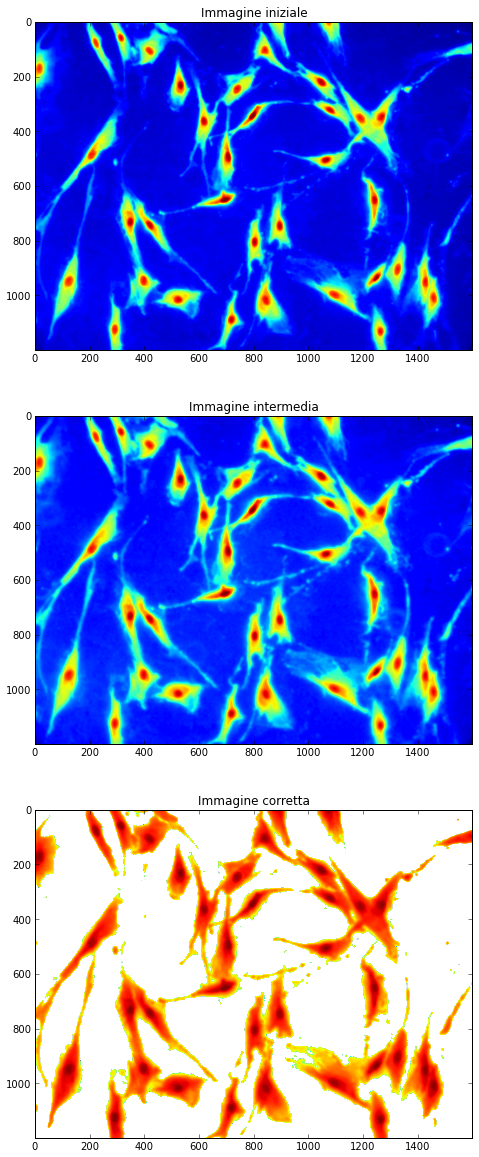
\includegraphics[scale=.50]{img/CAP4lg3.png}
 \caption{\small{Evoluzione dell'immagine delle cellule di fibroblasti: in alto è raffigurata l'immagine acquisita col microscopio a fluorescenza, al centro quella privata dei parametri costanti di background e in basso l'immagine risultante dopo aver corretto l'``effetto dei bordi''. Le immagini, rappresentate nella color map ``jet'' riportata a fianco, sono i logaritmi delle corrispettive immagini originali, a cui è stato applicato ulteriormente il filtro gaussiano.}}
 \label{fig:lg3}
\end{figure}

\begin{figure}
 \centering
 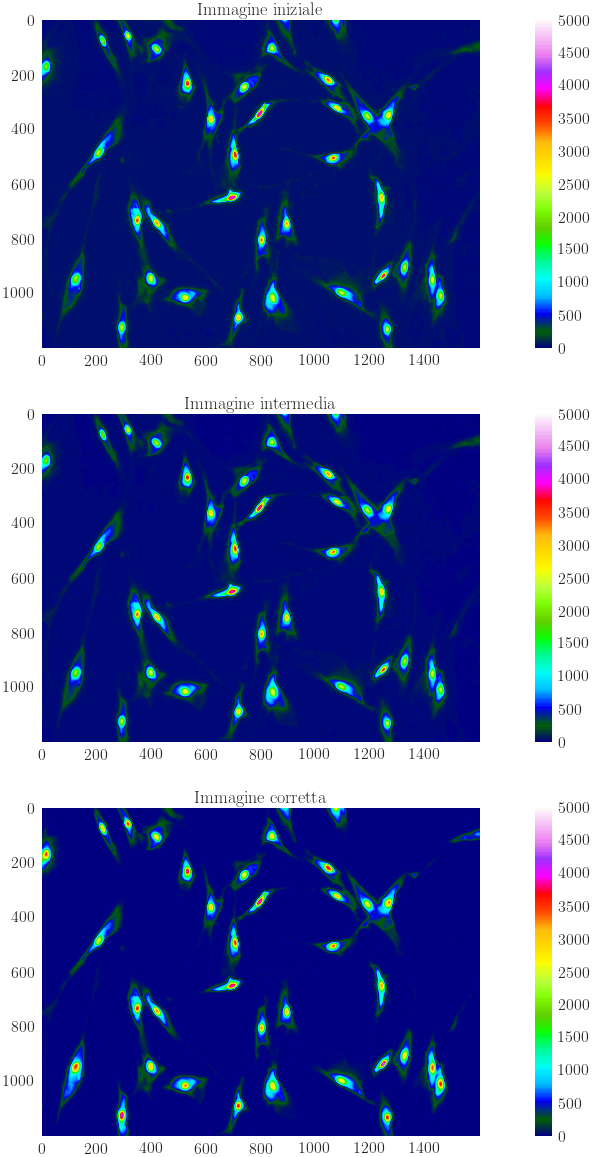
\includegraphics[scale=.50]{img/CAP4cmap.png}
 \caption{\small{Evoluzione dell'immagine delle cellule di fibroblasti: in alto è raffigurata l'immagine acquisita col microscopio a fluorescenza, al centro quella privata dei parametri costanti di background e in basso l'immagine risultante dopo aver corretto l'``effetto dei bordi''. Le immagini, rappresentate nella color map ``gist\_ncar'' riportata a fianco, sono le corrispettive immagini originali a cui è stato applicato il filtro gaussiano.}}
 \label{fig:cmap}
\end{figure}

Per quanto riguarda l'immagine delle cellule di fibroblasti, vero target dell'algoritmo di correzione, il cambiamento risulta davvero ben evidente: il difetto dei bordi è fortemente attenuato, infatti i nuclei più a margine riacquistano una colorazione molto più intensa e confrontabile con quella dei nuclei centrali, ed inoltre il background viene pressoché portato a zero, il tutto mantenendo ben definiti i confini delle varie cellule.
Le varie fasi correttive dell'immagini sono rappresentate sia in (\figurename~\ref{fig:lg3}) che in (\figurename~\ref{fig:cmap}).


\section{Confronto tra differenti immagini di calibrazione}

Come detto in precedenza, tale algoritmo permette la correzione dell'immagine a fluorescenza sulla base di due ulteriori immagini: la prima deve avere sferette di calibrazione a stessa intensità e viene sfruttata per la correzione dell'``effetto dei bordi'', mentre la seconda deve contenere sferette con differenti luminosità ed è necessaria per la rimozione del parametro di background. 
\'E sulla base di queste due ultime immagini che si ottengono i parametri necessari per la correzione di quella in esame.
Per tale motivo sono stati confrontati i risultati ottenuti con quattro distinte immagini di calibrazione ad una sola intensità: due con intensità relativa del 10\% (chiamate successivamente $10\%_1$ e $10\%_2$) e due con intensità relativa del 100\% (chiamate successivamente $100\%_1$ e $100\%_2$).

Dalle Figure \ref{fig:gauss1}, \ref{fig:gauss2}, \ref{fig:gauss3} e \ref{fig:gauss4} è evidente il fatto che differenti immagini di calibrazioni comportino differenti superfici tridimensionali risultanti dal fit di maximum likelihood, indipendentemente dall'intensità relativa delle sferette.

\begin{figure}
 \centering
 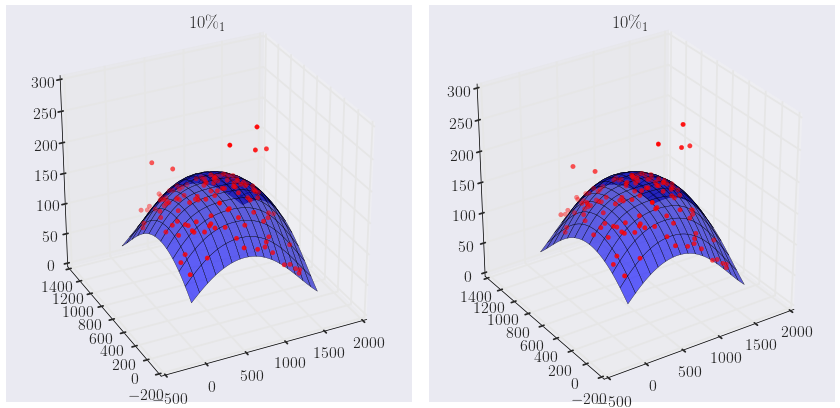
\includegraphics[scale=.45]{img/CAP4gauss1.png}
 \caption{\small{Immagine in visione ``cross eyed stereoscopic'' corrispondente alla prima immagine di calibrazione con intensità relativa del 10\%: i puntini rappresentano i massimi mentre la superficie è quella risultante dal fit di maximum likelihood.}}
 \label{fig:gauss1}
\end{figure}

\begin{figure}
 \centering
 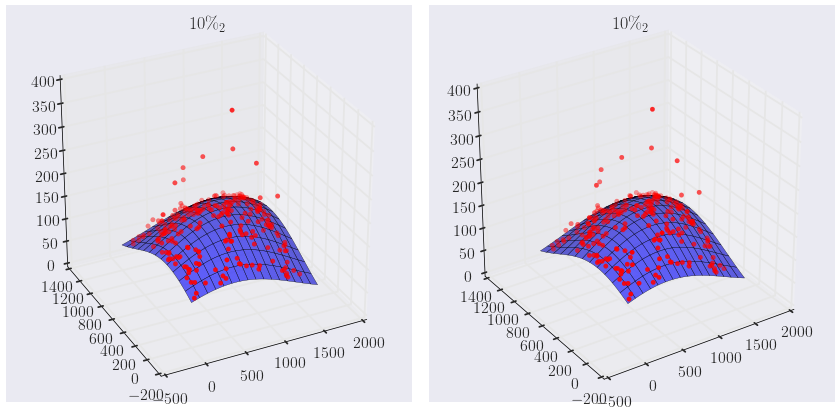
\includegraphics[scale=.45]{img/CAP4gauss2.png}
 \caption{\small{Immagine in visione ``cross eyed stereoscopic'' corrispondente alla seconda immagine di calibrazione con intensità relativa del 10\%: i puntini rappresentano i massimi mentre la superficie è quella risultante dal fit di maximum likelihood.}}
 \label{fig:gauss2}
\end{figure}

\begin{figure}
 \centering
 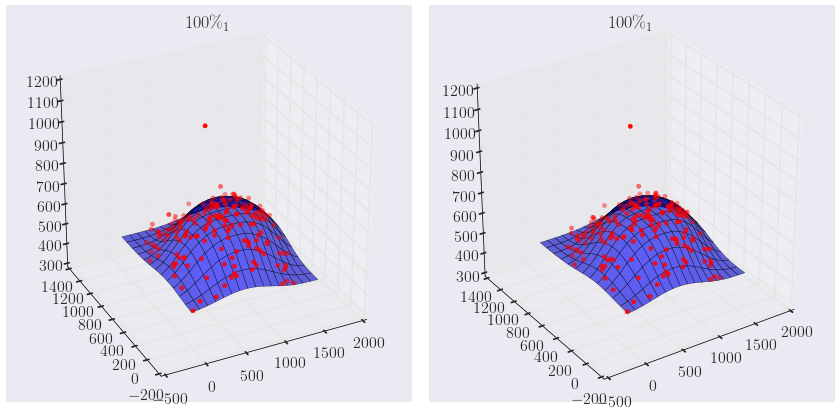
\includegraphics[scale=.45]{img/CAP4gauss3.png}
 \caption{\small{Immagine in visione ``cross eyed stereoscopic'' corrispondente alla prima immagine di calibrazione con intensità relativa del 100\%: i puntini rappresentano i massimi mentre la superficie è quella risultante dal fit di maximum likelihood.}}
 \label{fig:gauss3}
\end{figure}

\begin{figure}
 \centering
 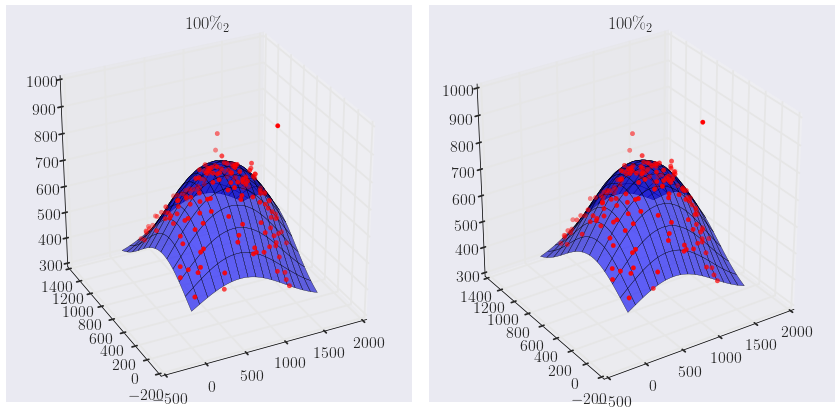
\includegraphics[scale=.45]{img/CAP4gauss4.png}
 \caption{\small{Immagine in visione ``cross eyed stereoscopic'' corrispondente alla seconda immagine di calibrazione con intensità relativa del 100\%: i puntini rappresentano i massimi mentre la superficie è quella risultante dal fit di maximum likelihood.}}
 \label{fig:gauss4}
\end{figure}

Per poter avere un'analisi di carattere più quantitativo sono stati visualizzati i parametri $bg,\ maxint,\ cx,\ cy,\ dsx,\ dsy,\ corr$ ed $e$ ottenuti dalla stima di massima verosimiglianza (capitolo 3.1) eseguita nei quattro casi (Figure \ref{fig:cx}, \ref{fig:cy}, \ref{fig:dsx}, \ref{fig:dsy} \ref{fig:bg}, \ref{fig:intmax}, \ref{fig:corr} e \ref{fig:e}).
Queste stime di massima verosimiglianza sono state inoltre raccolte nella \tablename~\ref{TABris}, assieme al primo parametro approssimato di background $bg_0$, calcolato inizialmente come massimo delle mode di ogni riga della matrice bidimensionale corrispondente all'immagine.

Dall'analisi di questi risultati si nota che differenti immagini di calibrazione comportano in genere differenti parametri, sebbene i valori si mantengano solitamente entro lo stesso ordine di grandezza.
Tuttavia per avere una miglior valutazione dell'effetto che tali differenze potrebbero comportare sulla correzione finale dell'immagine bisognerebbe eseguire elaborazioni successive, più raffinate rispetto alla semplice analisi qui riportata.

Nelle Figure \ref{fig:c1}, \ref{fig:c2}, \ref{fig:c3}, \ref{fig:c4} sono riportate le matrici di correlazione tra le stime dei parametri per le quattro differenti immagini di calibrazione.

\begin{table}
 \begin{center}
\begin{small}
\begin{tabular}{lcccc}
\hline\hline
&$\mathbf{10\%_1}$&$\mathbf{10\%_2}$&$\mathbf{100\%_1}$&$\mathbf{100\%_2}$\\
\hline
$\mathbf{bg_0}$& 19 & 19 & 13 & 13\\
\hline
$\mathbf{cx}$&$767\pm11$&$832\pm10$&$881\pm9$&$831\pm10$\\
$\mathbf{cy}$&$587\pm9$&$583\pm7$&$583\pm6 $&$608\pm6$\\
$\mathbf{dsx}$&$823\pm205$&$ 797\pm131$&$568 \pm17$&$663\pm66$\\
$\mathbf{dsy}$&$646\pm159$&$524\pm85$&$ 409\pm11$&$453\pm44$\\
$\mathbf{corr}$&$-0.29\pm0.06$&$-0.65\pm0.05 $&$-0.51\pm0.05$&$-0.49\pm0.05$\\
$\mathbf{bg}$&$1.58\cdot 10^{-6}\pm102$&$23\pm40 $&$452\pm13$&$341\pm82$\\
$\mathbf{maxint}$&$167\pm104$&$150\pm41$&$229\pm15$&$414\pm87$\\
$\mathbf{e}$&$3.2\pm0.6$&$2.1\pm0.3$&$3.6\pm0.4$&$2.5\pm0.4$\\
\hline\hline
\end{tabular}
\caption{\small{Confronto dei parametri ottenuti nella prima fase dell'algoritmo con quattro distinte immagini di calibrazione ad una sola intensità. Per ciascun parametro del fit vengono riportate la miglior stima e la deviazione standard associata, ottenute dalla procedura di fit. La precisione dei valori risulta elevata proprio poiché non si tratta di incertezze associate alla stima, bensì dei valori che approssimano localmente la funzione di likelihood con una distribuzione gaussiana.}}
\label{TABris}
\end{small}
\end{center}
\end{table}

\begin{figure}
 \centering
 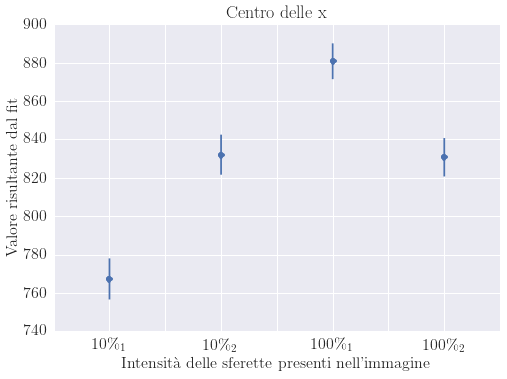
\includegraphics[scale=.50]{img/CAP4cx.png}
 \caption{\small{Parametro $cx$ (centro delle x) e intervallo di confidenza al 95\%, ottenuti tramite il fit di maximum likelihood presente nell'algoritmo, per le quattro differenti immagini di calibrazione ad una sola intensità.}}
 \label{fig:cx}
\end{figure}

\begin{figure}
 \centering
 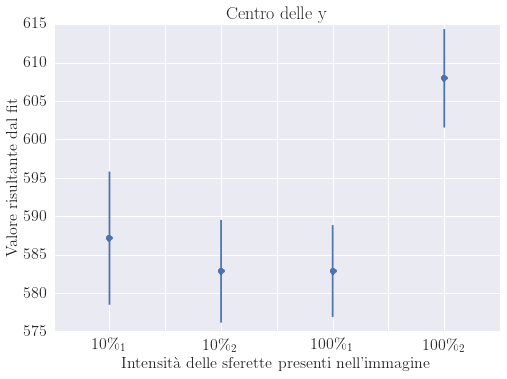
\includegraphics[scale=.50]{img/CAP4cy.png}
 \caption{\small{Parametro $cy$ (centro delle y) e intervallo di confidenza al 95\%, ottenuti tramite il fit di maximum likelihood presente nell'algoritmo, per le quattro differenti immagini di calibrazione ad una sola intensità.}}
 \label{fig:cy}
\end{figure}

\begin{figure}
 \centering
 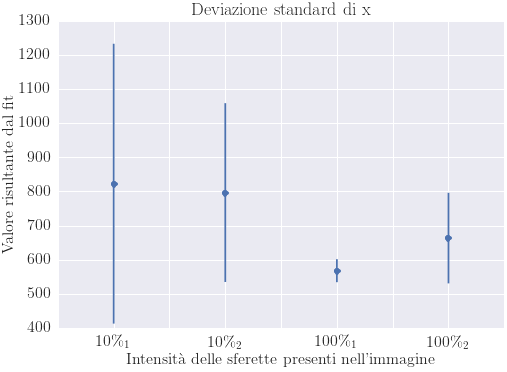
\includegraphics[scale=.50]{img/CAP4dsx.png}
 \caption{\small{Parametro $dsx$ (deviazione standard di x) e intervallo di confidenza al 95\%, ottenuti tramite il fit di maximum likelihood presente nell'algoritmo, per le quattro differenti immagini di calibrazione ad una sola intensità.}}
 \label{fig:dsx}
\end{figure}

\begin{figure}
 \centering
 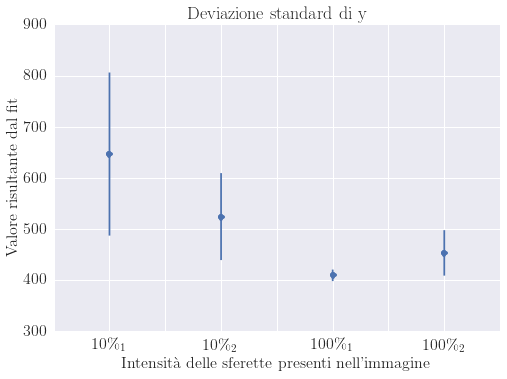
\includegraphics[scale=.50]{img/CAP4dsy.png}
 \caption{\small{Parametro $dsy$ (deviazione standard di y) e intervallo di confidenza al 95\%, ottenuti tramite il fit di maximum likelihood presente nell'algoritmo, per le quattro differenti immagini di calibrazione ad una sola intensità.}}
 \label{fig:dsy}
\end{figure}

\begin{figure}
 \centering
 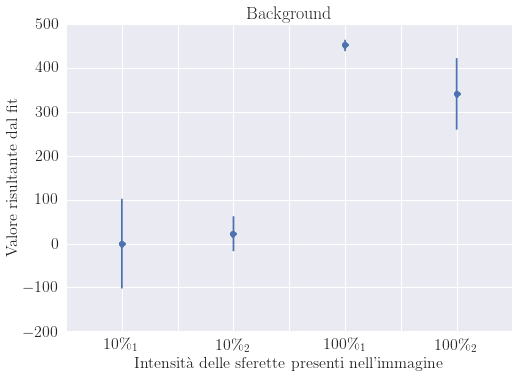
\includegraphics[scale=.50]{img/CAP4bg.png}
 \caption{\small{Parametro $bg$ (background) e intervallo di confidenza al 95\%, ottenuti tramite il fit di maximum likelihood presente nell'algoritmo, per le quattro differenti immagini di calibrazione ad una sola intensità.}}
 \label{fig:bg}
\end{figure}

\begin{figure}
 \centering
 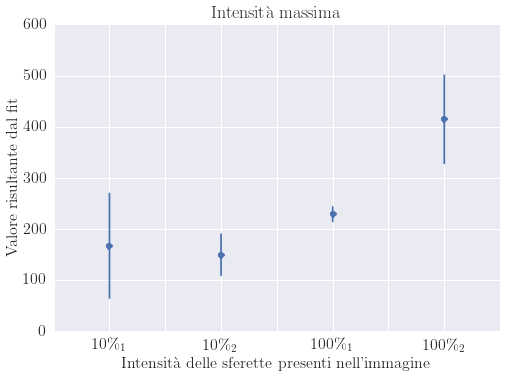
\includegraphics[scale=.50]{img/CAP4intmax.png}
 \caption{\small{Parametro $maxint$ (intensità massima) e intervallo di confidenza al 95\%, ottenuti tramite il fit di maximum likelihood presente nell'algoritmo, per le quattro differenti immagini di calibrazione ad una sola intensità.}}
 \label{fig:intmax}
\end{figure}

\begin{figure}
 \centering
 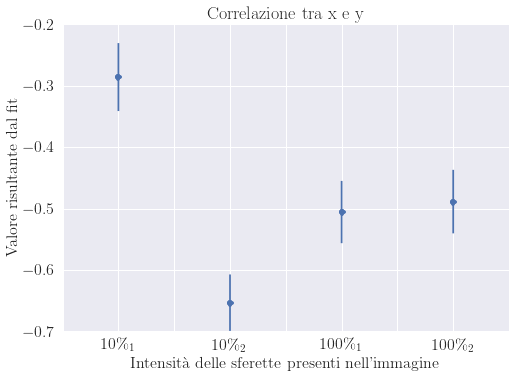
\includegraphics[scale=.50]{img/CAP4corr.png}
 \caption{\small{Parametro $corr$ (correlazione tra x ed y) e intervallo di confidenza al 95\%, ottenuti tramite il fit di maximum likelihood presente nell'algoritmo, per le quattro differenti immagini di calibrazione ad una sola intensità.}}
 \label{fig:corr}
\end{figure}

\begin{figure}
 \centering
 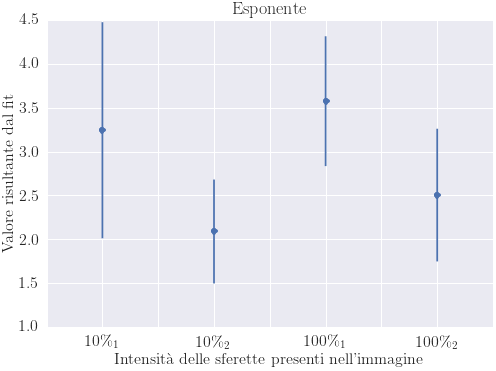
\includegraphics[scale=.50]{img/CAP4e.png}
 \caption{\small{Parametro $e$ (esponente) e intervallo di confidenza al 95\%, ottenuti tramite il fit di maximum likelihood presente nell'algoritmo, per le quattro differenti immagini di calibrazione ad una sola intensità.}}
 \label{fig:e}
\end{figure}

\begin{figure}
 \centering
 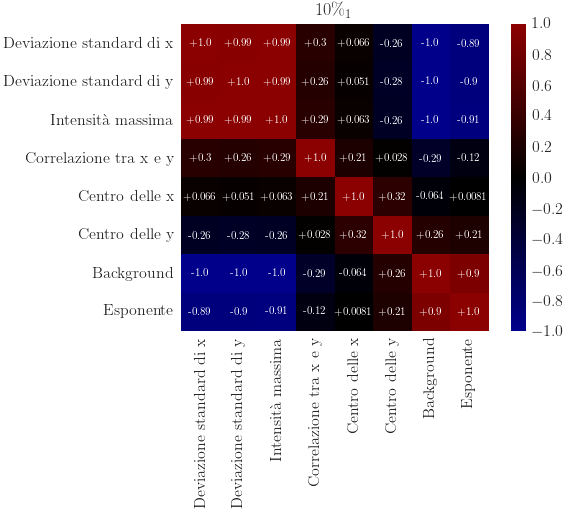
\includegraphics[scale=.45]{img/CAP4c1.png}
 \caption{\small{Matrice di correlazione tra le stime dei parametri ottenuti dal fit di maximum likelihood per l'immagine di calibrazione $10\%_1$.}}
 \label{fig:c1}
\end{figure}

\begin{figure}
 \centering
 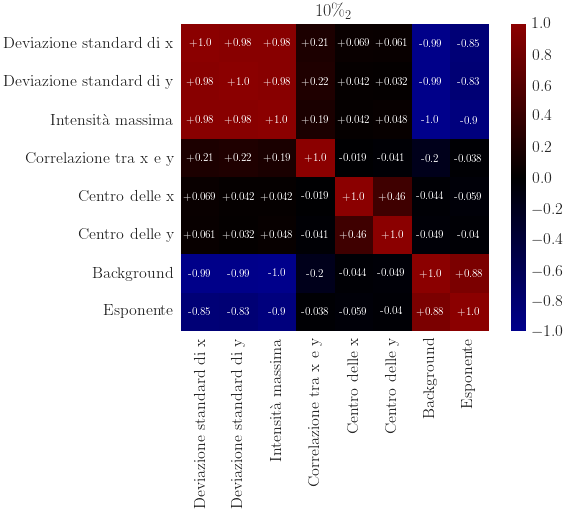
\includegraphics[scale=.45]{img/CAP4c2.png}
 \caption{\small{Matrice di correlazione tra le stime dei parametri ottenuti dal fit di maximum likelihood per l'immagine di calibrazione $10\%_2$.}}
 \label{fig:c2}
\end{figure}

\begin{figure}
 \centering
 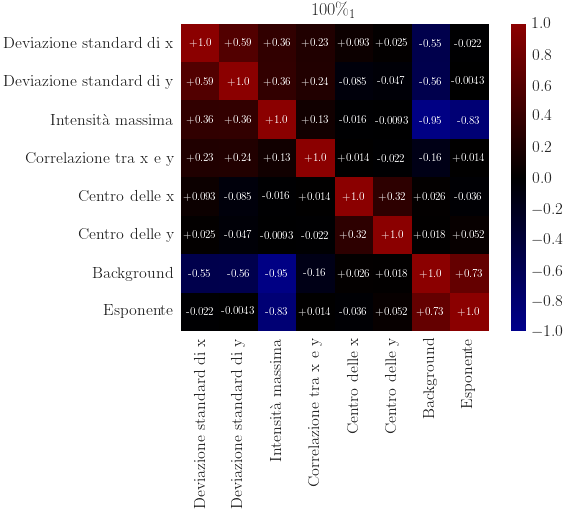
\includegraphics[scale=.45]{img/CAP4c3.png}
 \caption{\small{Matrice di correlazione tra le stime dei parametri ottenuti dal fit di maximum likelihood per l'immagine di calibrazione $100\%_1$.}}
 \label{fig:c3}
\end{figure}

\begin{figure}
 \centering
 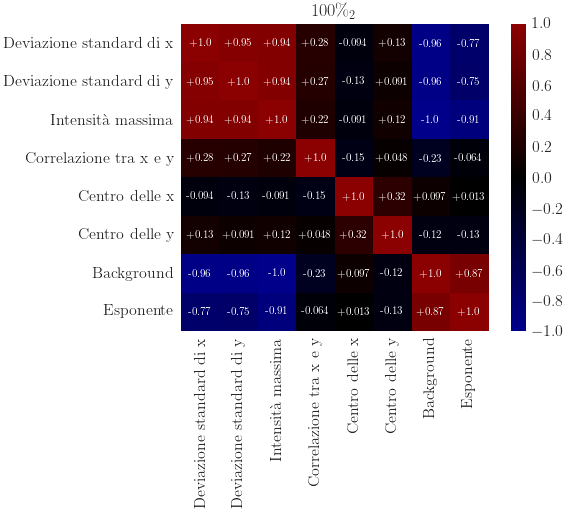
\includegraphics[scale=.45]{img/CAP4c4.png}
 \caption{\small{Matrice di correlazione tra le stime dei parametri ottenuti dal fit di maximum likelihood per l'immagine di calibrazione $100\%_2$.}}
 \label{fig:c4}
\end{figure}


